\chapter{转换结果分析}

\section{IEEE9网络}

\begin{figure}[H]
\centering
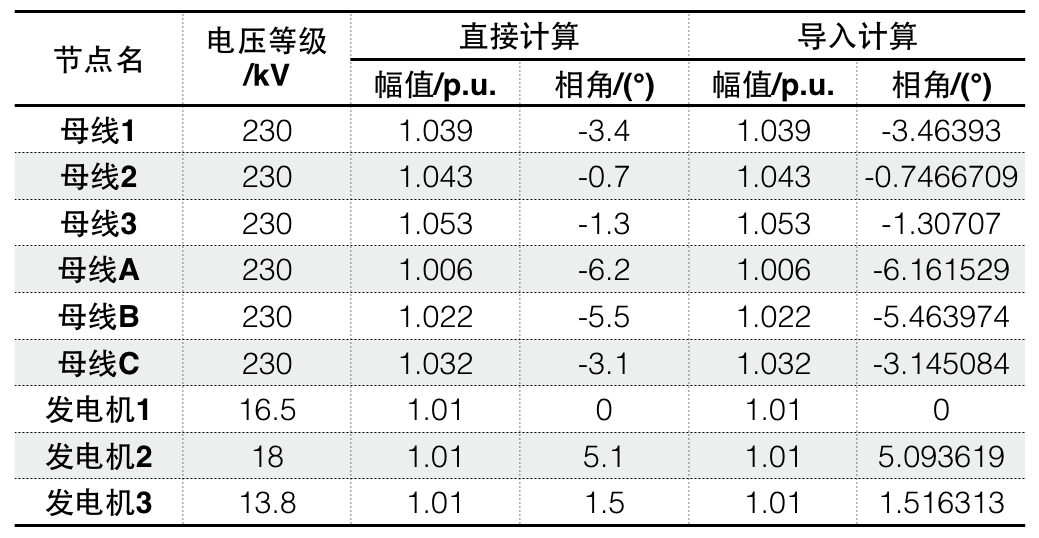
\includegraphics[width=1.05\textwidth]{images/Paper_Fig_55.png}
\setcaptionwidth{\linewidth}
\caption{IEEE9潮流计算结果比较}
\end{figure}

图6.1所示为3机9节点系统在 DIgSILENT中直接建模和通过由 BPA 模型自动转换和导入 DIgSILENT 两种数据导入方式下 3机 9节点系统在DIgSILENT仿真软件中的潮流计算结果。由图6.1可见,两种数据导入方式下的潮流计算结果基本一致,微小的差异主要由于模型转化过程中数据保留的有效位数不同所致。

\section{IEEE39网络}

\begin{figure}[H]
\centering
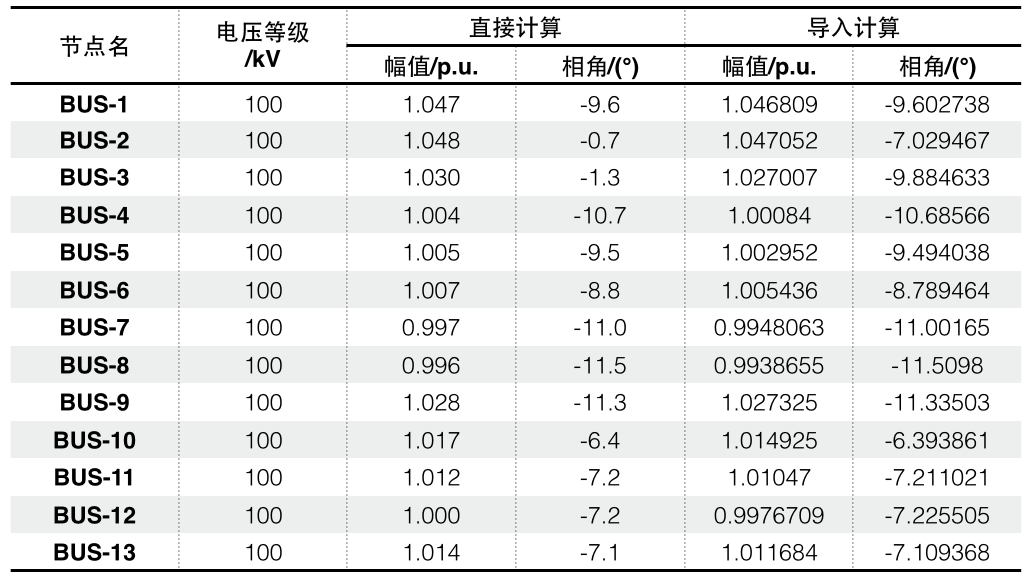
\includegraphics[width=1.0\textwidth]{images/Paper_Fig_56.png}
\setcaptionwidth{\linewidth}
\caption{IEEE39潮流计算结果比较}
\end{figure}

\begin{figure}[H]
\centering
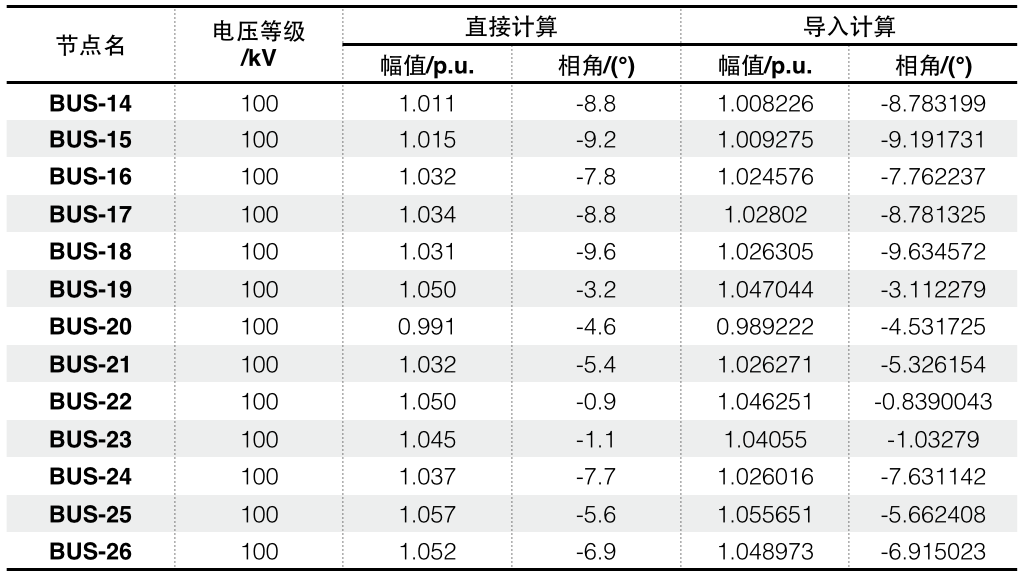
\includegraphics[width=1.0\textwidth]{images/Paper_Fig_57.png}
\setcaptionwidth{\linewidth}
\caption{IEEE39潮流计算结果比较}
\end{figure}

\begin{figure}[H]
\centering
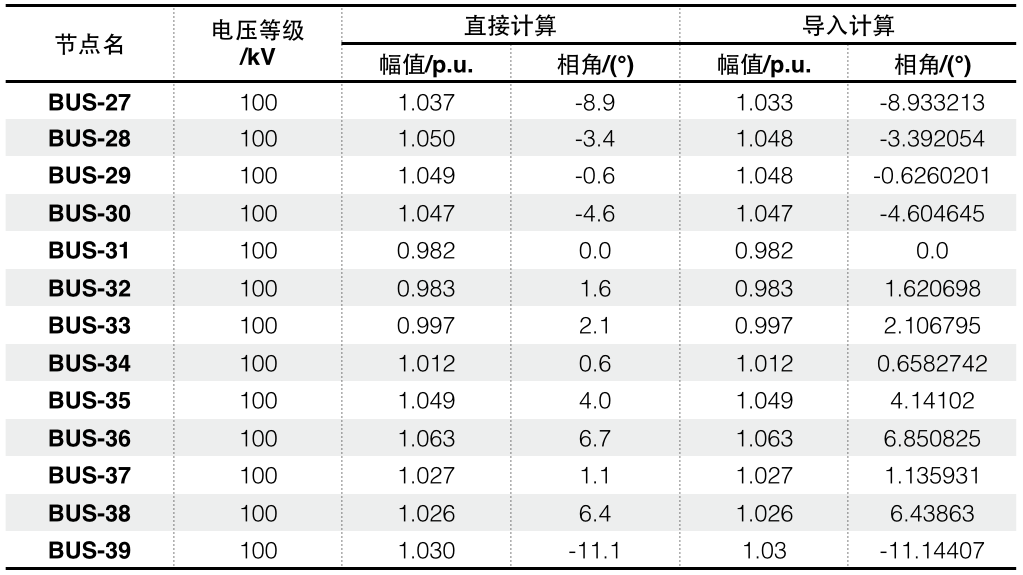
\includegraphics[width=1.0\textwidth]{images/Paper_Fig_58.png}
\setcaptionwidth{\linewidth}
\caption{IEEE39潮流计算结果比较}
\end{figure}

\begin{figure}[H]
\centering
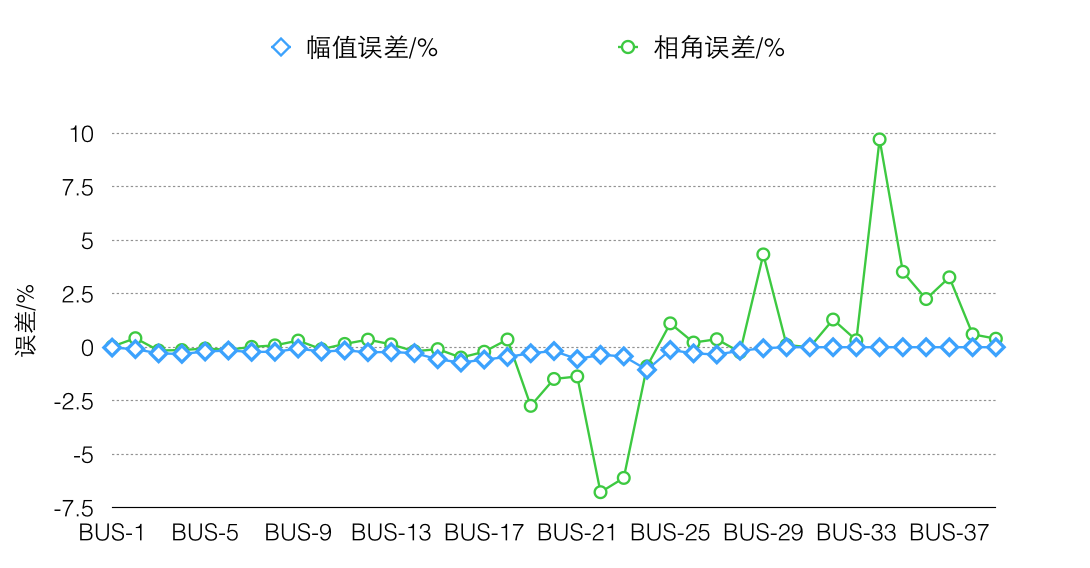
\includegraphics[width=1.0\textwidth]{images/Paper_Fig_59.png}
\setcaptionwidth{\linewidth}
\caption{转换结果误差比较}
\end{figure}

图6.2、6.3、6.4、6.5所示为IEEE39节点系统在 DIgSILENT中直接建模和通过由 BPA 模型自动转换和导入 DIgSILENT 两种数据导入方式下IEEE39节点系统在DIgSILENT仿真软件中的潮流计算结果,从中可以看出:

\begin{description}[1cm]
\item[-] 两种方式下的潮流计算结果基本一致
\item[-] 相比于幅值结果,相角误差相对较大
\item[-] 微小的差异主要由于模型转化过程中数据保留的有效位数不同所致
\end{description}

综上所述,误差在允许范围内,BPA导入DIgSILENT数据转换程序的开发达到了设计要求。
